\subsection{Datenbank und Persistenz\label{subsec:datenbank}}
%TODO Kapitel schreiben


\subsubsection{Konfiguration des Glassfish AS zur Verwendung einer MySQL Datenbank}

\subsection{Datenmodell und Datenbankschema}
Die Datenbank wurde nach dem \enquote{Code first} Ansatz entwickelt.
Diese Vorgehensweise wurde gewählt, da das bisherige Datenmodell erweitert wurde und die Datenbank nach belieben angepasst werden kann, da keine anderen Anwendungen direkt auf die Datenbank zugreifen.

Das Datenmodell besteht aus \ac{JPA}"~Entitätsklassen (Entity). 
Dies sind mit \ac{JPA}"~Annotationen versehene \ac{POJO}-Klassen sind \cite[vgl.][17-19]{Keith.2013}.

Das resultierende Datenbankschema (siehe Abbildung \ref{fig:datenmankschema}) wird durch den \ac{ORM}"~Provider erstellt und bedarf keine manuellen Anpassungen, da Schlüssel, Beziehungen und Einschränkungen der Tabellen direkt in den Entitätsklassen mit Annotationen festgelegt werden können.

Lediglich eine View wurde manuell erstellt, um die Vorgabe des Authentifizierungsproviders zu erfüllen (siehe Abschnitt \ref{subsubsec:anmeldedaten_datenbank})

\begin{minipage}[t]{\textwidth}
	\centering
	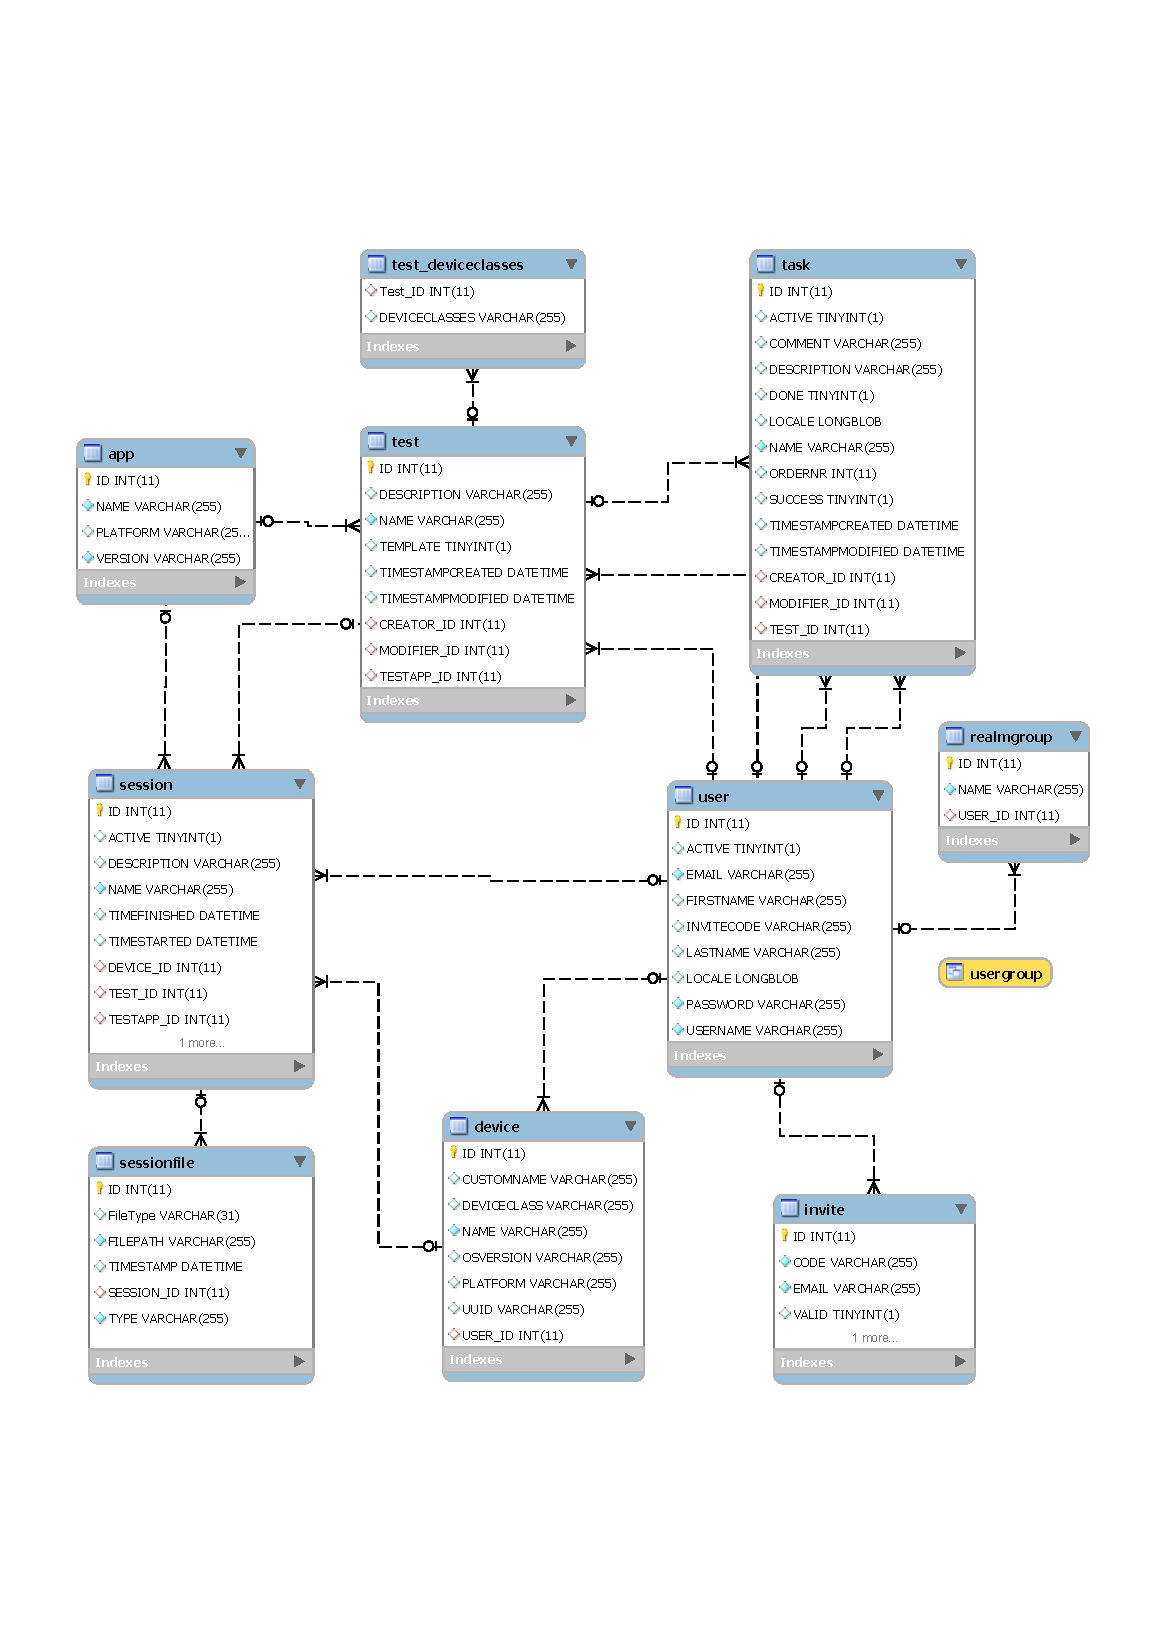
\includegraphics[width=\linewidth]{img/datenbankschema}
	\captionof{figure}{Datenbankschema des Hipsterbility-Servers.}
	\label{fig:datenmankschema}
\end{minipage}

\begin{minipage}[t]{\textwidth}

\begin{tabu}{|>{\ttfamily}X>{\ttfamily}X>{\small}X[2]|}
\everyrow{\hline}
\hline
\rowfont[l]{\normalfont\bfseries} 
Datenbanktabelle & Entitätsklasse(n) & Beschreibung \\ 
app & TestAppEntity & Eine im System registrierte Applikation die für Test vorgesehen ist \\ 
device & DeviceEntity & Registrierte Geräte der Benutzer \\ 
user & UserEntity & Benutzerdaten und Sammlungen von Objekten mit Benutzerbezug \\ 
realmgroup & GroupEntity & Rollenzuweisung der Benuter \\ 
invite & InviteEntity & Einladung für die Registrierung neuer Benutzer \\ 
session & TestSessionEntity & Repräsentation eines durchgeführten Testdurchlaufs \\ 
test & TestEntity & Objekt zur Darstellung eines Usability-Tests \\ 
task & TaskEntity & Eine Aufgabe in einem Usability-Test, welche vom Testbenutzer ausgeführt werden soll. \\ 
test\_deviceclasses & \emph{DeviceClass} String enum & Eine Liste mit Geräteklassen für die der jeweilige Test durchgeführt werden soll. \\ 
sessionfile & FileEntity \normalfont{Subklassen} & Tabelle mit Pfaden und Metainformationen zu Dateien, die vom Android-Client während einer Testsitzung erstellt werden \\ 

\end{tabu} 
\label{tbl:tabellen_und_entities}
\captionof{table}{Tabellen und Entitäten der Persiszenzschicht.}
\end{minipage}